%%%%%%%%%%%%%%%%%%%%%%%%%%%%%%%%%%%%%%%%%
% Programming/Coding Assignment
% LaTeX Template
%
% This template has been downloaded from:
% http://www.latextemplates.com
%
% Original author:
% Ted Pavlic (http://www.tedpavlic.com)
%
% Note:
% The \lipsum[#] commands throughout this template generate dummy text
% to fill the template out. These commands should all be removed when 
% writing assignment content.
%
% This template uses a Perl script as an example snippet of code, most other
% languages are also usable. Configure them in the "CODE INCLUSION 
% CONFIGURATION" section.
%
%%%%%%%%%%%%%%%%%%%%%%%%%%%%%%%%%%%%%%%%%

%----------------------------------------------------------------------------------------
%	PACKAGES AND OTHER DOCUMENT CONFIGURATIONS
%----------------------------------------------------------------------------------------

\documentclass{article}

\usepackage{fancyhdr} % Required for custom headers
\usepackage{lastpage} % Required to determine the last page for the footer
\usepackage{extramarks} % Required for headers and footers
\usepackage[usenames,dvipsnames]{color} % Required for custom colors
\usepackage{graphicx} % Required to insert images
\usepackage{listings} % Required for insertion of code
\usepackage{courier} % Required for the courier font
\usepackage{lipsum} % Used for inserting dummy 'Lorem ipsum' text into the template
\usepackage[utf8]{inputenc}
\usepackage[ngerman]{babel}

% Margins
\topmargin=-0.45in
\evensidemargin=0in
\oddsidemargin=0in
\textwidth=6.5in
\textheight=9.0in
\headsep=0.25in

\linespread{1.1} % Line spacing

% Set up the header and footer
\pagestyle{fancy}
\lhead{\hmwkAuthorName} % Top left header
\chead{\hmwkClass\ : \hmwkTitle} % Top center head
\rhead{\firstxmark} % Top right header
\lfoot{\lastxmark} % Bottom left footer
\cfoot{} % Bottom center footer
\rfoot{Page\ \thepage\ of\ \protect\pageref{LastPage}} % Bottom right footer
\renewcommand\headrulewidth{0.4pt} % Size of the header rule
\renewcommand\footrulewidth{0.4pt} % Size of the footer rule

\setlength\parindent{0pt} % Removes all indentation from paragraphs

%----------------------------------------------------------------------------------------
%	CODE INCLUSION CONFIGURATION
%----------------------------------------------------------------------------------------

\definecolor{MyDarkGreen}{rgb}{0.0,0.4,0.0} % This is the color used for comments
\lstloadlanguages{Perl} % Load Perl syntax for listings, for a list of other languages supported see: ftp://ftp.tex.ac.uk/tex-archive/macros/latex/contrib/listings/listings.pdf
\lstset{language=Perl, % Use Perl in this example
        frame=single, % Single frame around code
        basicstyle=\small\ttfamily, % Use small true type font
        keywordstyle=[1]\color{Blue}\bf, % Perl functions bold and blue
        keywordstyle=[2]\color{Purple}, % Perl function arguments purple
        keywordstyle=[3]\color{Blue}\underbar, % Custom functions underlined and blue
        identifierstyle=, % Nothing special about identifiers                                         
        commentstyle=\usefont{T1}{pcr}{m}{sl}\color{MyDarkGreen}\small, % Comments small dark green courier font
        stringstyle=\color{Purple}, % Strings are purple
        showstringspaces=false, % Don't put marks in string spaces
        tabsize=5, % 5 spaces per tab
        %
        % Put standard Perl functions not included in the default language here
        morekeywords={rand},
        %
        % Put Perl function parameters here
        morekeywords=[2]{on, off, interp},
        %
        % Put user defined functions here
        morekeywords=[3]{test},
       	%
        morecomment=[l][\color{Blue}]{...}, % Line continuation (...) like blue comment
        numbers=left, % Line numbers on left
        firstnumber=1, % Line numbers start with line 1
        numberstyle=\tiny\color{Blue}, % Line numbers are blue and small
        stepnumber=5 % Line numbers go in steps of 5
}

% Creates a new command to include a perl script, the first parameter is the filename of the script (without .pl), the second parameter is the caption
\newcommand{\perlscript}[2]{
\begin{itemize}
\item[]\lstinputlisting[caption=#2,label=#1]{#1.pl}
\end{itemize}
}

%----------------------------------------------------------------------------------------
%	DOCUMENT STRUCTURE COMMANDS
%	Skip this unless you know what you're doing
%----------------------------------------------------------------------------------------

% Header and footer for when a page split occurs within a problem environment
\newcommand{\enterProblemHeader}[1]{
%\nobreak\extramarks{#1}{#1 continued on next page\ldots}\nobreak
%\nobreak\extramarks{#1 (continued)}{#1 continued on next page\ldots}\nobreak
}

% Header and footer for when a page split occurs between problem environments
\newcommand{\exitProblemHeader}[1]{
%\nobreak\extramarks{#1 (continued)}{#1 continued on next page\ldots}\nobreak
%\nobreak\extramarks{#1}{}\nobreak
}

\setcounter{secnumdepth}{0} % Removes default section numbers
\newcounter{homeworkProblemCounter} % Creates a counter to keep track of the number of problems

\newcommand{\homeworkProblemName}{}
\newenvironment{homeworkProblem}[1][Problem \arabic{homeworkProblemCounter}]{ % Makes a new environment called homeworkProblem which takes 1 argument (custom name) but the default is "Problem #"
\stepcounter{homeworkProblemCounter} % Increase counter for number of problems
\renewcommand{\homeworkProblemName}{#1} % Assign \homeworkProblemName the name of the problem
\section{\homeworkProblemName} % Make a section in the document with the custom problem count
\enterProblemHeader{\homeworkProblemName} % Header and footer within the environment
}{
\exitProblemHeader{\homeworkProblemName} % Header and footer after the environment
}

\newcommand{\problemAnswer}[1]{ % Defines the problem answer command with the content as the only argument
\noindent\framebox[\columnwidth][c]{\begin{minipage}{0.98\columnwidth}#1\end{minipage}} % Makes the box around the problem answer and puts the content inside
}

\newcommand{\homeworkSectionName}{}
\newenvironment{homeworkSection}[1]{ % New environment for sections within homework problems, takes 1 argument - the name of the section
\renewcommand{\homeworkSectionName}{#1} % Assign \homeworkSectionName to the name of the section from the environment argument
\subsection{\homeworkSectionName} % Make a subsection with the custom name of the subsection
\enterProblemHeader{\homeworkProblemName\ [\homeworkSectionName]} % Header and footer within the environment
}{
\enterProblemHeader{\homeworkProblemName} % Header and footer after the environment
}

%----------------------------------------------------------------------------------------
%	NAME AND CLASS SECTION
%----------------------------------------------------------------------------------------

\newcommand{\hmwkTitle}{Übung\ \#1} % Assignment title
\newcommand{\hmwkDueDate}{Montag,\ 20.\ Oktober\ 2014} % Due date
\newcommand{\hmwkClass}{Reconfigurable Embedded Systems} % Course/class
\newcommand{\hmwkClassTime}{} % Class/lecture time
\newcommand{\hmwkClassInstructor}{} % Teacher/lecturer
\newcommand{\hmwkAuthorName}{Günther Schindler} % Your name

%----------------------------------------------------------------------------------------
%	TITLE PAGE
%----------------------------------------------------------------------------------------

\title{
\vspace{2in}
\textmd{\textbf{\hmwkClass:\ \hmwkTitle}}\\
\normalsize\vspace{0.1in}\small{Abgabe\ am\ \hmwkDueDate}\\
\vspace{0.1in}\large{\textit{\hmwkClassTime}}
\vspace{3in}
}

\author{\textbf{\hmwkAuthorName}}
\date{} % Insert date here if you want it to appear below your name

%----------------------------------------------------------------------------------------

\begin{document}

\maketitle

%----------------------------------------------------------------------------------------
%	TABLE OF CONTENTS
%----------------------------------------------------------------------------------------

%\setcounter{tocdepth}{1} % Uncomment this line if you don't want subsections listed in the ToC

\newpage
\tableofcontents
\newpage

%----------------------------------------------------------------------------------------
%	PROBLEM 1
%----------------------------------------------------------------------------------------

% To have just one problem per page, simply put a \clearpage after each problem

\begin{homeworkProblem}[D-latch]
Das D-latch ist ein 1-Bit Datenspeicher.
\begin{center}
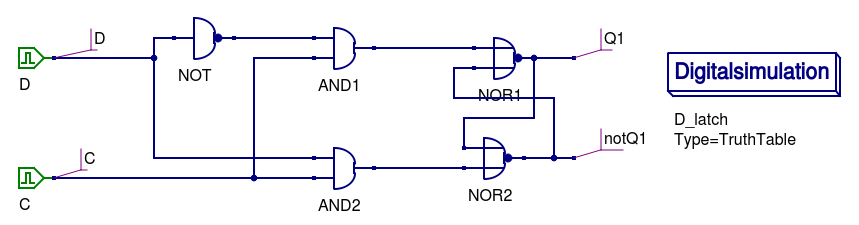
\includegraphics[width=0.6\columnwidth]{dlatch_schem}
\end{center}
Der Ausgang (Q1) folgt dem Dateneingang (D) sofern der Enable-Eingang (C) gleich 1 ist. Ist der
Enable-Eingang gleich 0, wird der vorige Wert gespeichert. Ist der Enable-Eingang gleich 0 zu einem Zeitpunkt in dem noch kein Wert durch den
Dateneingang gespeichert wurde, ist der Ausgang undefiniert (X).
\begin{center}
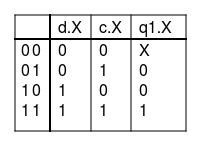
\includegraphics[width=0.2\columnwidth]{dlatch_truth}
\end{center}
\end{homeworkProblem}

%Listing \ref{homework_example} shows a Perl script.

%\perlscript{homework_example}{Sample Perl Script With Highlighting}

%\lipsum[1]

%----------------------------------------------------------------------------------------
%	PROBLEM 2
%----------------------------------------------------------------------------------------

\begin{homeworkProblem}[Decoder]
Ein Decoder ist ein Umsetzer für digitale Signale. So können beispielsweise 2 Eingangssignale auf 4 Ausgangssignale umgesetzt werden.
Nachfolgende Schaltung zeigt eine Realisierung eines 4-aus-2-Decoders um die Eingangsadressen auf entsprechende Ausgangswerte (siehe Logiktabelle)
umzusetzen.
\begin{center}
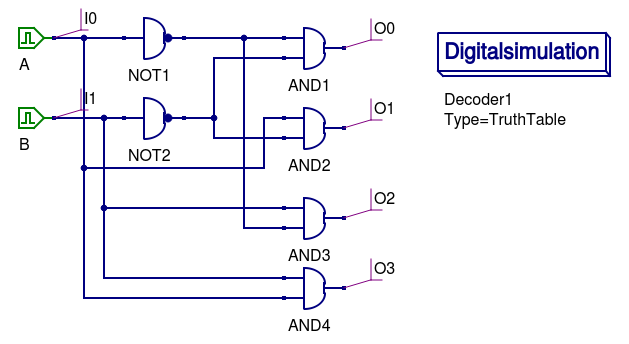
\includegraphics[width=0.6\columnwidth]{decoder1_schem}
\end{center}
\begin{center}
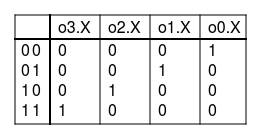
\includegraphics[width=0.3\columnwidth]{decoder1_truth}
\end{center}
\end{homeworkProblem}

\begin{homeworkProblem}[Multiplexer]
Multiplexer sind Selektionsschalter, die digitale Eingangssignale auf einen Ausgang durchschalten können. Nachfolgende Schaltung zeigt eine
Realisierung um aus zwei Eingangssignalen (D0, D1) ein Signal auswählen zu können. Die Auswahl erfolgt mittels Select-Eingang (S) und kann mit
dem Enable-Eingang (E) aktiviert werden.
\begin{center}
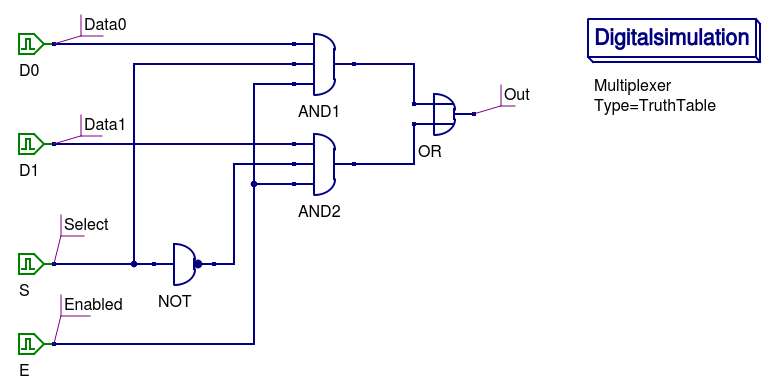
\includegraphics[width=0.6\columnwidth]{mux_schem}
\end{center}
\begin{center}
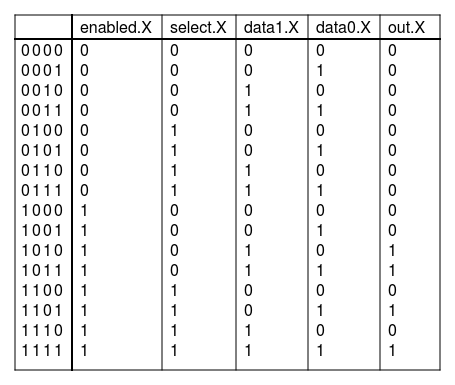
\includegraphics[width=0.3\columnwidth]{mux_truth}
\end{center}
Diese Schaltung eines Multiplexers ergibt in idealisierter Form (d.h. ohne Komponentenverzögerung) folgendes Zeitverlaufsdiagramm.
\begin{center}
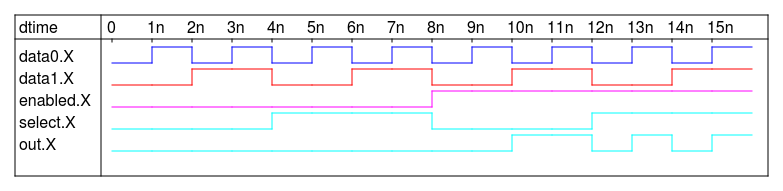
\includegraphics[width=0.8\columnwidth]{mux_time}
\end{center}
\end{homeworkProblem}

\clearpage
\begin{homeworkProblem}[16-Bit Multiplexer]
Ein einfacher 2-zu-1 Multiplexer kann mithilfe von vier 2-input NAND-Gates realisiert werden. Wie nachfolgendes Bild zeigt, ergibt sich die
komplette Schaltzeit über drei Stufen. Bei einer Verzögerung von 10ns je Gate, ergibt sich eine gesamte Verzögerung von 30ns für diesen 2-Bit MUX.
%\begin{figure}[htb]
\begin{center}
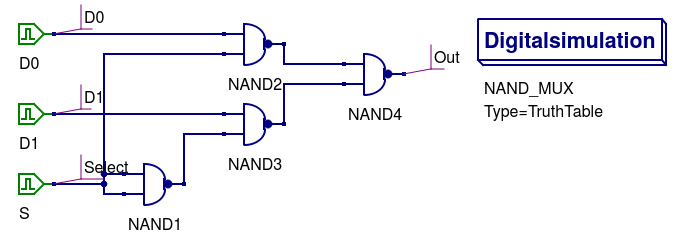
\includegraphics[width=0.6\columnwidth]{2to1MUX}
\end{center}
Wird der 16-Bit Multiplexer mit einer Reihe von 2-Bit Multiplexern realisiert, ergibt sich die Schaltzeit über vier Stufen. 
\begin{center}
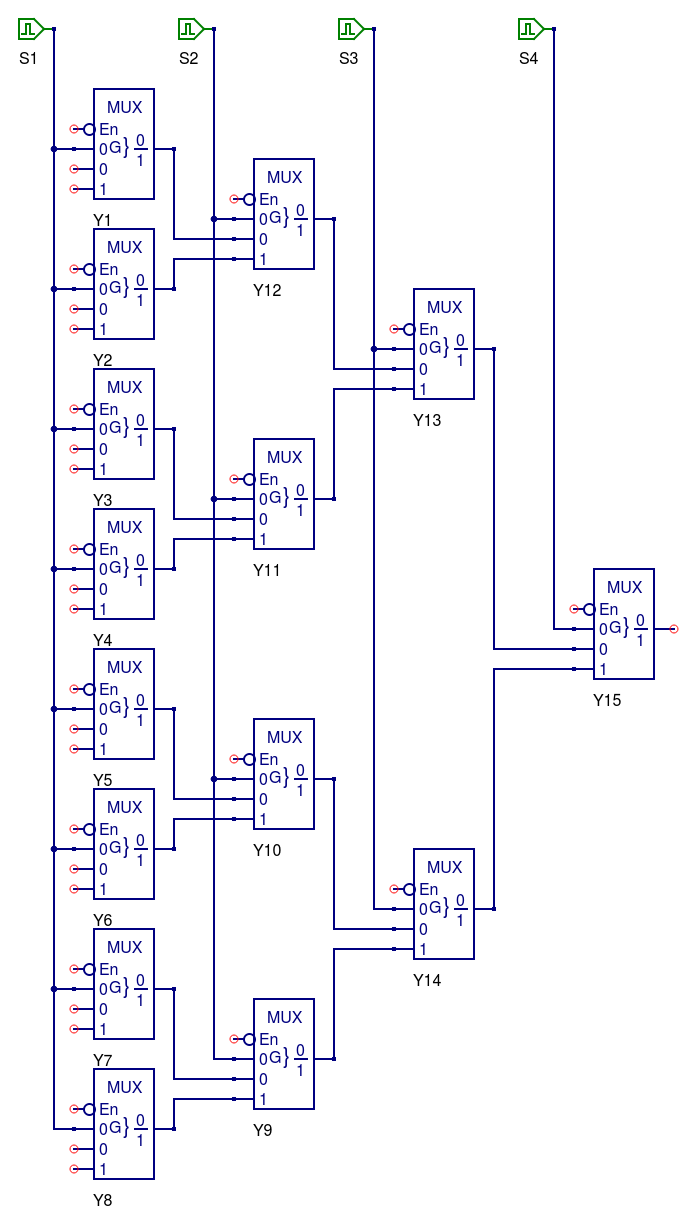
\includegraphics[width=0.3\columnwidth]{16bitMUX} 
\end{center}
Bei einer Verzögerung von 30ns je 2-Bit Multiplexer ergibt sich eine Verzögerung von 30ns je Stufe und somit eine gesamte Verzögerung von 120ns
für den 16-Bit Multiplexer.
\newline
\newline
Versucht man diese Schaltung mit einem Takt von 20ns zu betreiben, wird man nicht zum gewünschten Ergebnis kommen, da die 2-Bit Multiplexer
mindestens 30ns zum verarbeiten der Daten brauchen. Um die Schaltung trotzdem mit einer Taktquelle von 20ns betreiben zu können, benötigt man
zusätzlich eine Komponente die den Takt verlangsamt. Deispielsweise könnte man dies mithilfe eines positiv-flankengesteuertes JK-FlipFlops realisieren. Bei der
Eingangskombination J=K=1 wechselt das FlipFlop bei jedem Taktimpuls seinen Zustand (toggle). Jede Stufe des FlipFlops halbiert also den Takt.
\begin{center}
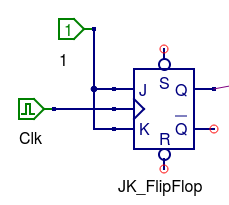
\includegraphics[width=0.15\columnwidth]{JK}
\end{center}
\end{homeworkProblem}
\begin{homeworkProblem}[SN74ALVC08 und SN74ALVH374]
Das SN74ALVC08 ist ein vierfaches UND Gatter mit je zwei Eingängen und positiver Logik. Der Baustein dient zur logischen UND verknüpfung von
zwei Eingängen.
\newline
Das SN74ALVH374 ist ein achtfach flanken-getriggertes D-FlipFlop. Bei positiver Taktflanke des CLK-Eingangs wird der Q-Ausgang auf das logische
Level des Dateneingangs (D) gesetzt.
\newline
Die Gatterlaufzeit (propagation delay) beträgt bei dem SN74ALVC08 bei einer Betriebsspannung von 3.3V minimal 1.2ns und maximal 2.9ns. Bei dem 
SN74ALVH374 beträgt die Gatterlaufzeit bei gleicher Betriebsspannung minimal 1.1ns und maximal 3.6ns.
\newline
Verzögerungszeiten wie Tplz usw. beziehen sich auf Pegeländerungen vom Z-Zustand in den H- oder L-Zustand bzw. vom H- oder L-Zustand in den
Z-Zustand. Tplz und Tphz werden als Output disable time from low level bezeichnet. Tpzh und Tpzl werden als Output enable time to high level
bezeichnet.
\newline
Die Setup-Time (Zeit, für die sich ein Eingangssignal vor der aktiven Schaltflanke des Taktsignals nicht ändern darf) beträgt bei dem SN74ALVH374
1.8ns. Im Datenblatt des SN74ALVC08 wurde die Setup-Time nicht mit angegeben.
\end{homeworkProblem}

\begin{homeworkProblem}[LPC800 mini board]
Im Schaltplan des LPC800 mini boards finden sich passive Komponenten (Widerstände und Kondensatoren) und auch nichtlineare Komponenten (Dioden
und Transistoren). Die Linien zwischen diesen Komponenten symbolisieren Verbindungen. In Kombination ergeben sich Netzwerke, die die
Spannungs- und Stromverhältnisse bei den Schaltvorgängen verbessern. Versorgt werden die Komponenten mit Spannungswerten von 3.3V und 5V.
\newline
Neben einem Mini-USB-Anschluss findet sich auch ein USB-RS232-Interface-Chip, der eine serielle Kommunikation via USB ermöglicht.
\newline
Die zentrale Komponente dieser Schaltung ist ein LPC800 Microcontroller.
\end{homeworkProblem}



%----------------------------------------------------------------------------------------

\end{document}